%!TEX root = ../template.tex
%%%%%%%%%%%%%%%%%%%%%%%%%%%%%%%%%%%%%%%%%%%%%%%%%%%%%%%%%%%%%%%%%%%%
%% chapter1.tex
%% NOVA thesis document file
%%
%% Chapter 1: Introduction
%%%%%%%%%%%%%%%%%%%%%%%%%%%%%%%%%%%%%%%%%%%%%%%%%%%%%%%%%%%%%%%%%%%%

\typeout{NT FILE chapter1.tex}%

\chapter{Introduction}
\label{cha:introduction}

\section{Motivation}
\label{sec:intro_motivation}

Software systems are complex socio-technical artefacts that must evolve under technical, organisational, and human constraints. In this setting, software and conceptual modelling provide structured abstractions that can support reasoning, communication, and early validation before implementation \cite{buchmann2019conceptual}. In higher education, modelling is therefore commonly taught in software engineering and related programmes through notations and methods such as UML, BPMN, ER, or goal-oriented requirements approaches \cite{istar-learning,bpmn-education,maslov2025conceptual}.

Despite its recognised importance, students often perceive modelling in polarised ways: as a valuable instrument for understanding and communicating about systems, or as burdensome ``extra documentation'' that competes with implementation time \cite{chakraborty2022perceptions,grassl2026dei,liebel2017model}. These perceptions are shaped by course-level conditions and by how modelling is situated within the learning workflow---for example, the tools used, the nature of modelling tasks and domains, the role of models in assessment, and how feedback is provided \cite{grassl2026dei,liebel2017model}. Understanding how such conditions relate to modelling practice and competence development is important for improving modelling education and for fostering modelling skills that transfer beyond individual course contexts \cite{maslov2025conceptual}.


\section{Problem statement and research gap}
\label{sec:intro_gap}

Research on modelling education has produced valuable insights, but evidence and concepts are distributed across different modelling traditions and study contexts \cite{maslov2025conceptual}. Prior work has (i) proposed outcome-oriented frameworks and taxonomies that help articulate modelling competencies and highlight recurring gaps (e.g., limited explicit attention to evaluation and metacognitive aspects) \cite{bogdanova2019camelot,bogdanova2017domain,bork2019framework}, and (ii) reported, in method- and course-specific empirical studies, recurring difficulties such as grasping construct meaning, moving from requirements to models, and judging model adequacy, often alongside suggestions for pedagogical or tool-mediated support \cite{istar-learning,bpmn-education}.

However, there remains a need for an integrated, empirically grounded understanding of modelling education challenges and support needs that reflects both student and instructor viewpoints across educational contexts, and that connects reported difficulties to the socio-technical conditions in which modelling is taught and practiced \cite{liebel2017model,maslov2025conceptual}.

\section{Aim and research questions}
\label{sec:intro_aim_rq}

The aim of this thesis is to develop an empirically grounded account of modelling education challenges and support needs in higher education, treating modelling as a socio-technical activity that combines conceptual understanding, procedural strategies, and contextual influences.

The study is guided by the following research questions:

\begin{itemize}
    \item \textbf{RQ1:} What challenges do students and instructors perceive in learning and teaching software modelling in higher education, and how do these challenges manifest across different modelling activities (e.g., interpreting, creating, refining, and evaluating models)?
    \item \textbf{RQ2:} What strategies do students and instructors employ to address these challenges, and what support needs (pedagogical and tool-related) do they identify?
    \item \textbf{RQ3:} How do socio-technical factors (e.g., tools, course design, domains, feedback practices) shape modelling learning and teaching experiences?
\end{itemize}

In line with these questions, the analysis focuses respectively on (RQ1) challenges as they appear across modelling activities, (RQ2) coping strategies and articulated support needs, and (RQ3) the socio-technical conditions that shape how modelling is learned and taught.

\section{Research approach overview}
\label{sec:intro_approach}

To address these questions, the thesis adopts a qualitative, theory-building approach. The study is conducted using Grounded Theory, informed by a socio-technical stance that attends to interactions between social and technical elements in modelling education \cite{hoda2018socio,stol2016grounded}. Data are collected from students and instructors through semi-structured interviews, complemented by task- or artefact-anchored elicitation to ground reflections in concrete modelling practice \cite{istar-learning}. Bloom's revised taxonomy is used as a sensitising concept to help communicate the cognitive character of reported challenges without constraining the grounded analysis \cite{krathwohl2002revision,stol2016grounded}. The primary outcome is a grounded explanatory account of modelling learning and teaching challenges and associated support needs; secondarily, the thesis derives implications and design-oriented recommendations for teaching practice and educational tool support.

\section{Expected contributions}
\label{sec:intro_contributions}

This thesis contributes to software and conceptual modelling education research in four complementary ways. First, it provides an empirically grounded characterisation of the challenges that students and instructors perceive in learning and teaching modelling, including difficulties that arise across different modelling activities such as interpreting problem descriptions, constructing models, refining them, and judging their quality.

Second, it offers an integrated account of the strategies participants use to cope with these challenges and the support needs they articulate. These support needs span pedagogical practices (e.g., scaffolding, feedback, assessment framing) and tool-mediated support (e.g., guidance, feedback on errors, and mechanisms for managing complexity), and are derived from concrete examples elicited during interviews and activity- or artefact-centred discussion.

Third, the thesis develops a socio-technical explanatory perspective that links modelling challenges and coping strategies to contextual factors such as tool ecosystems, course design choices, feedback practices, and assignment domains. This perspective is intended to clarify how modelling experiences are shaped by interactions between cognitive demands and the educational settings in which modelling is taught and practiced.

Finally, the thesis provides evidence-informed implications for modelling education design. These implications are formulated as actionable recommendations for instructors and course designers and as requirements-level insights for those developing educational modelling tools, with the goal of supporting modelling competence that is robust beyond individual course contexts.


\section{Thesis structure}
\label{sec:intro_structure}

The remainder of this thesis is structured as follows. Chapter~\ref{cha:background} provides background on software and conceptual modelling, modelling education, grounded theory, Bloom-based learning outcomes, and human factors relevant to modelling learning. Chapter~\ref{cha:related_work} reviews related work on modelling education frameworks, empirical studies of modelling learning challenges, tooling and model-driven engineering in education, and contextual factors such as motivation, inclusion, and authenticity. Chapter~\ref{cha:methodology} presents the research design, research questions, data collection and analysis procedures, and considerations of rigour, ethics, and limitations. Subsequent chapters present the findings and discuss implications for modelling education and tool support.

%!TEX root = ../template.tex
%%%%%%%%%%%%%%%%%%%%%%%%%%%%%%%%%%%%%%%%%%%%%%%%%%%%%%%%%%%%%%%%%%%%
%% chapter2.tex
%% NOVA thesis document file
%%
%% Chapter 2: Background
%%%%%%%%%%%%%%%%%%%%%%%%%%%%%%%%%%%%%%%%%%%%%%%%%%%%%%%%%%%%%%%%%%%%

\typeout{NT FILE chapter2.tex}%

\chapter{Background}
\label{cha:background}

\section{Software modelling \& conceptual modelling}
\label{sec:software_modelling_conceptual}

\subsection{Purpose and role of modelling in software engineering}
\label{subsec:purpose_role_modelling_se}


Software modelling supports reasoning about software systems by creating representations that abstract from reality to emphasise aspects that matter for a given purpose and audience. In software engineering, models can serve multiple roles: they may act as design blueprints, facilitate communication among stakeholders, and enable analysis and validation of properties before implementation \cite{buchmann2019conceptual,maslov2025conceptual}.

A useful clarification is that modelling should not be reduced to producing diagrammatic pictures. Rather, models are structured artefacts expressed in a modelling language with defined meaning, and their usefulness depends on what they represent and how they are intended to be used. Kühne highlights that the term \emph{model} is often used ambiguously, and proposes a distinction between \emph{type models} (the modelling languages or model types that define what can be expressed) and \emph{token models} (the concrete model instances created for a particular problem) \cite{kuhne:DagSemProc.04101.15}. This distinction helps explain why learning modelling involves more than symbol recognition: it requires understanding the language-level concepts and constraints (type level) and being able to construct, adapt, and assess concrete models for specific tasks (token level).

\subsection{Conceptual modelling as a broader discipline}
\label{subsec:conceptual_modelling_broader_discipline}

It is useful to distinguish between software modelling as a practice within software engineering and conceptual modelling as a broader discipline concerned with representing, structuring, and reasoning about domains and systems across fields. Conceptual modelling is not limited to software development alone; it is also used in organisational analysis, enterprise and service design, data-intensive systems, and other domains where abstraction is needed to manage complexity and support understanding \cite{maslov2025conceptual}. Reviews of conceptual modelling education underline its interdisciplinary nature and identify a broad family of modelling subtypes---including data, process, goal, and enterprise modelling---that often evolve in parallel, with limited pedagogical or theoretical integration across subfields \cite{bogdanova2019camelot,bogdanova2017domain,maslov2025conceptual}.

This disciplinary perspective is particularly relevant for research on teaching and learning software modelling. When modelling is treated primarily as a supplementary topic within software engineering courses, students may not fully appreciate its significance and may develop oversimplified views of its purpose and applicability. In contrast, the conceptual modelling perspective frames modelling languages as knowledge schemas: they define what can be expressed, how meaning is structured, and what kinds of analysis or tooling become possible. Understanding modelling therefore requires engaging with notational elements and underlying semantics, as well as modelling goals and the intended audience of the produced model artefacts \cite{buchmann2019conceptual}.

\subsection{Modelling methods, languages, and artefacts}
\label{subsec:modelling_methods_languages_artefacts}

Several authors emphasise that a modelling method is more than a set of symbols or a notation. A modelling method can be understood as comprising a modelling language (including syntax, semantics, and notation), a modelling procedure (the process or steps to create models), and supporting mechanisms and algorithms such as analysis, simulation, or transformation capabilities \cite{bork2019framework,buchmann2019conceptual}. This holistic view clarifies why students may be able to reproduce diagrammatic symbols yet still struggle to apply modelling meaningfully: the procedural and analytical aspects of modelling are often less explicitly taught or assessed.

From this viewpoint, the value of a modelling language is not only in enabling representation, but also in supporting reasoning. When a language is treated as a structured schema, models become more than static diagrams: they can become queryable, analysable, and transformable artefacts that enable deeper engagement with a domain. This also motivates tool support that can provide feedback on syntactic correctness, highlight semantic issues, help manage complexity, or automate parts of modelling tasks \cite{bogdanova2019camelot,maslov2025conceptual}.

\subsection{Implications for the scope of this thesis}
\label{subsec:implications_scope_thesis}

This thesis adopts the view that software modelling is an instantiation of the broader discipline of conceptual modelling. It therefore treats modelling as a discipline involving conceptual understanding of modelling constructs and their semantics, procedural competence in constructing and refining model artefacts from problem descriptions, analytical judgement of model quality and fit-for-purpose, and socio-technical awareness of how modelling practices are shaped by tools, learning contexts, and stakeholder needs. This framing aligns with work on modelling learning outcomes and competencies, which emphasises not only notational knowledge but also procedural skills, evaluative abilities, and reflective understanding \cite{bogdanova2019camelot,bogdanova2017domain,bork2019framework,sedelmaier2013research}. This perspective motivates the subsequent background on modelling education, grounded theory, and learning outcomes, and provides a foundation for investigating modelling challenges from both student and instructor perspectives.

\section{Modelling education}
\label{sec:modelling_education}

\subsection{Overview of conceptual modelling education}
\label{subsec:overview_conceptual_modelling_education}

Conceptual and software modelling are widely taught across computing and software-related programmes, but they are taught in diverse ways and appear in different course contexts and curricular roles. Maslov et al.\ \cite{maslov2025conceptual} map the conceptual modelling education literature and show that educational work spans multiple modelling sub-communities (e.g., data modelling, process modelling, enterprise modelling), which have developed partially independent emphases, terminology, and pedagogical traditions \cite{maslov2025conceptual}. Within this landscape, modelling appears in contexts ranging from introductory courses to advanced software engineering modules, and courses emphasise different modelling families and purposes (e.g., data-centric, process-centric, goal-oriented).

The same studies also highlight that much practice in modelling education is shaped by instructor experience and local institutional constraints, as well as by the availability of tools, rather than by systematically articulated educational frameworks or empirically validated design principles \cite{maslov2025conceptual}. While there is broad consensus on the importance of modelling skills for software professionals, there is less agreement on which specific \emph{competencies} learners should acquire, how these competencies should be scaffolded, and how learning should be assessed in a reliable and educationally meaningful way.

\subsection{Bloom-based perspectives on modelling learning outcomes}
\label{subsec:bloom_perspectives_modelling_learning_outcomes}

To make modelling learning outcomes more explicit and comparable across courses and contexts, several authors have proposed adaptations of Bloom's revised taxonomy for conceptual and domain modelling. Starting from Bloom’s six cognitive process categories---\emph{remember}, \emph{understand}, \emph{apply}, \emph{analyse}, \emph{evaluate}, and \emph{create} \cite{krathwohl2002revision}---these works operationalise them in modelling terms. Typical modelling-specific interpretations include recalling notation elements and rules (remember), explaining construct meaning and purpose (understand), constructing models by applying modelling rules and procedures to a problem description (apply), checking models for consistency/completeness and identifying defects (analyse), judging model quality and comparing alternatives against criteria (evaluate), and producing or extending models and modelling solutions for new situations (create).

Bogdanova and Snoeck analyse learning outcomes and assessment tasks for domain modelling through the lens of Bloom's revised taxonomy, reporting that many tasks concentrate on \emph{understanding}, \emph{analysing}, and \emph{creating} \emph{conceptual knowledge}, while giving less explicit attention to \emph{evaluation} activities and to \emph{procedural} and \emph{metacognitive} knowledge \cite{bogdanova2017domain}. Notably, across Bloom-informed modelling frameworks the mapping between Bloom categories, modelling tasks, and knowledge types is not uniform (some works emphasise cognitive processes, others additionally foreground the knowledge dimension); however, a recurring observation is the relative underrepresentation of evaluation and reflective/metacognitive aspects in current educational practice.

Bork extends this Bloom-based perspective to both conceptual modelling and metamodeling, mapping knowledge and cognitive dimensions to all components of a modelling method (language, semantics, notation, procedure, mechanisms and algorithms) \cite{bork2019framework}. An evaluation of a ``Smart City'' teaching case using this framework reveals that even rich, practice-oriented material may still underemphasise certain cognitive levels (e.g., evaluation) or knowledge types (e.g., metacognitive knowledge). These works collectively suggest that Bloom's taxonomy can provide a useful lens for reflecting on and improving modelling education, by making learning objectives more explicit and balanced across different dimensions.

\subsection{Process and goal modelling education}
\label{subsec:process_goal_modelling_education}

Beyond data and structural modelling, there is growing interest in how students learn process and goal-oriented modelling. For business process modelling with BPMN, Maslov outlines a research agenda for developing empirically validated process-modelling education that integrates insights from conceptual modelling education, process model quality research, and learning sciences \cite{bpmn-education}. This agenda highlights the need for systematic mapping of existing work, empirical studies of novice modellers' behaviour and typical errors, and the design and experimental evaluation of BPMN-specific teaching strategies and feedback mechanisms. This reflects a broader recognition that teaching process modelling effectively requires more than just introducing notation; it requires attention to cognitive demands, quality criteria, and the kinds of feedback needed to help learners improve.

Goal-oriented requirements modelling approaches introduce additional layers of complexity, as it requires learners to reason about stakeholder intentions, rationales, and dependencies. An iStar learning study explicitly investigates the challenges students face when learning iStar, using a combination of Bloom-based task framing and grounded theory analysis of tutorials, modelling sessions, and interviews \cite{istar-learning}. The authors report difficulties at multiple cognitive levels, including understanding the semantics of iStar constructs, applying the notation to real requirements, and analysing models to assess completeness and appropriateness. They derive a catalogue of strategies and tool-supported requirements (e.g., conceptual clarification, syntax checking, process guidance, templates, visualisation, and semi-automation modelling from text) that could help address these challenges \cite{istar-learning}.

These strands of work on BPMN and iStar education illustrate that different modelling families pose distinct learning challenges and may require specialised pedagogical approaches. They also reinforce broader themes in modelling education, including the need for scaffolding from text to model, support for managing complexity, and explicit attention to how learners evaluate and refine their models.

\subsection{Modelling, tools, and model-driven engineering in education}
\label{subsec:tools_mde_education}

Modelling in educational settings is often mediated by tools, ranging from simple drawing tools and web-based modellers to industrial-grade model-driven engineering (MDE) environments. Tool choice can influence students' perceptions of modelling and their opportunities to practice particular skills. Liebel et al.\ conducted a multi-case study of model-driven software engineering courses that use different tools (e.g., Umple, Papyrus) and place different emphasis on model-driven architecture and code generation \cite{liebel2017model}. Their results indicate that students' perceptions of tools are highly context-dependent: the same tool may be perceived positively in one course setup and negatively in another, depending on project design, available support, and the roles that models play (e.g., for communication versus strict code generation). They also find that perceptions of UML as modelling language are more positive and robust when models are used for requirements and analysis, rather than only as precise inputs to code generators \cite{liebel2017model}.

These findings align with broader discussions of human factors in model-driven engineering, which argue that educational tools should prioritise usability, cognitive support, constructive feedback, and alignment with learning goals over industrial feature completeness \cite{human-factors-mde}. From an educational perspective, this suggests that tool selection and integration should be carefully considered to ensure they support the intended modelling competencies and do not inadvertently increase cognitive load or distract from learning objectives.

\subsection{Competence-oriented and human-centred perspectives}
\label{subsec:competence_human_centre}

Broader software engineering education research brings in complementary competence-oriented and human-centred perspectives that can inform modelling education. Sedelmaier and Landes propose the EVELIN research agenda for identifying and developing required competencies in software engineering, arguing that curricula should be grounded in explicit competence models rather than only topic lists \cite{sedelmaier2013research}. They introduce a six-level classification system (remember, understand, explain, use, apply, develop) for technical competencies and outline an iterative, data-driven approach to relating teaching methods and structural conditions to competency development \cite{sedelmaier2013research}. This approach resonates with the Bloom-based frameworks discussed earlier, but emphasises the need for empirical validation and alignment with real-world professional requirements.

Work on human factors in modelling and software engineering education further highlights the role of motivation, inclusion, and authenticity. For example, studies on domain diversity and motivation in modelling courses show that educators' assumptions about which domains are motivating (e.g., games, automation) do not always match students' preferences, and that students value domains that connect to their interests and everyday or socially relevant contexts \cite{grassl2026dei}. Students also report that feeling excluded by unfamiliar or culturally distant domains, or by assignment setups that do not fit their backgrounds, can hinder their engagement and learning \cite{grassl2026dei}. More generally, experiential education initiatives emphasise the value of working on real systems, real tasks, and with real mentors to bridge the gap between classroom modelling exercises and the complexities of practice \cite{holmes2018dimensions}.

Taken together, these competence-oriented and human-centred perspectives reinforce the idea that modelling education should be designed not only around notations and tools, but also around the competencies to be developed, the diversity of learners, and the authenticity and inclusiveness of modelling tasks and domains.

\subsection{Implications for this thesis}
\label{subsec:modelling_education_implications}

The literature on modelling education, Bloom-based frameworks, process and goal modelling, tooling, competencies, and human factors provides several important implications for this thesis. First, it suggests that modelling learning outcomes can be systematically described in terms of cognitive and knowledge dimensions, and that existing courses may underemphasise evaluation and metacognitive aspects of modelling competence \cite{bogdanova2019camelot, bogdanova2017domain, bork2019framework}. Second, it shows that different modelling families (e.g., data, process, goal) can pose partly distinct learning demands and error patterns, meaning that findings are not automatically transferable across notations and tasks. At the same time, family-specific empirical studies—such as the iStar learning work—provide a useful methodological precedent for how to elicit challenges in a task-anchored way and derive support requirements grounded in learner experience, which this thesis adapts to a broader educational scope. \cite{istar-learning, bpmn-education}. Third, it highlights that tools and model-driven approaches can both enable and hinder learning, depending on how they are integrated into course designs and on the kind of feedback and affordances they provide \cite{liebel2017model,human-factors-mde}. Finally, competence-oriented and human-centred research indicates that modelling education must be sensitive to students' motivations, backgrounds, and learning environments, and that explicit competence models can support more systematic design and evaluation of teaching \cite{chakraborty2022perceptions,holmes2018dimensions,sedelmaier2013research}.

These insights inform the research questions and methodological choices of this thesis, which aims to investigate how students and teachers experience modelling, which challenges they perceive, and what kinds of support may foster the development of modelling competencies in realistic educational contexts.


\section{Grounded Theory}
\label{sec:grounded_theory}

\subsection{Overview and key characteristics}
\label{subsec:gt_overview}

Grounded Theory (GT) is a qualitative research methodology originally developed in sociology with the aim of generating theory that is systematically grounded in data rather than deduced from prior hypotheses. Instead of starting from a fixed theoretical framework, GT proceeds iteratively: data collection and analysis occur simultaneously, and emerging insights guide subsequent sampling and questioning. Core practices include \emph{coding} (assigning conceptual labels to segments of data), \emph{constant comparison} (comparing new data with existing codes and categories), and \emph{theoretical sampling} (collecting new data to refine or challenge emerging concepts), and extensive \emph{memoing} to capture analytic ideas \cite{adolph2011using,stol2016grounded}. 

The outcome of a GT study is not a set of descriptive themes, but a more abstract, integrated explanation of how participants handle a central problem or concern. This explanation is typically organised around a \emph{core category} that captures a dominant pattern in the data and links other categories together. Evaluation criteria emphasise the \emph{fit} of concepts to the data, the \emph{workability} of the emerging theory in explaining the studied phenomenon, its \emph{relevance} to practitioners and researchers, and its \emph{modifiability} in light of new data, rather than statistical notions of validity \cite{adolph2011using}.

Over time, GT has evolved into several variants, including \emph{Classic GT} (Glaser and Strauss), \emph{Straussian GT} (Strauss and Corbin), and \emph{Constructivist GT} (Charmaz) \cite{charmaz2006constructing,glaser1967discovery,strauss1998basics}. While these variants share core principles, they differ in the degree to which they prescribe specific coding procedures, the role of prior theory, and the epistemological stance of the researcher. For software engineering research, this diversity offers flexibility but also introduces risks of inconsistent or superficial use if methodological choices are not made explicit \cite{stol2016grounded}.

\subsection{Grounded Theory in software engineering}
\label{subsec:gt_in_se}

In software engineering (SE), GT has been used to study topics that are difficult to capture through controlled experiments or surveys, such as developer experience, team practices, decision-making processes, and socio-technical phenomena. A critical review by Stol et al.\ \cite{stol2016grounded} finds that GT has become increasingly popular in SE research, but that many studies lack methodological rigour, adopt only parts of GT procedures, and show limited reflexivity regarding the researcher's role \cite{stol2016grounded}. To address these issues, they offer a set of guidelines on when GT is appropriate (e.g., for under-theorised, practice-oriented problems), how to choose among GT variants, and how to report GT studies in a way that allows readers to assess their quality.

Adolph et al.\ provide a concrete example of applying classical (Glaserian) GT to study how software practitioners cope with the process of development, while also reflecting on the practical challenges of conducting GT research in SE contexts \cite{adolph2011using}. They describe in detail how they conducted open coding on interviews and field observations, developed concepts and categories through constant comparison, and iteratively refined their sampling strategy to explore interesting phenomena in more depth. Their work highlights the importance of staying close to the data, avoiding overly mechanical use of qualitative analysis tools, and systematically documenting analytic decisions through memos.

These contributions establish GT as a suitable methodology for SE when the research goal is to generate mid-level substantive theory about human and organisational aspects of software development, and they provide concrete guidance for designing and reporting such studies.

\subsection{Socio-Technical Grounded Theory}
\label{subsec:stgt}

Hoda et al.\ propose Socio-Technical Grounded Theory (STGT) as a specialisation of GT for SE that explicitly foregrounds the socio-technical nature of software development \cite{hoda2018socio}. STGT retains the core principles of GT (iterative data collection and analysis, constant comparison, theoretical sampling, memoing) but emphasises the need to attend simultaneously to social and technical elements and their interactions. This involves, for example, paying attention to roles, norms, tools, artefacts, and organisational structures, and analysing how these co-evolve over time.

STGT also articulates expectations for rigour in terms of credibility, transferability, dependability, and confirmability, and provides detailed guidance on reporting, including the description of research context, participants, data sources, coding procedures, and the evolution of categories and core concepts \cite{hoda2018socio}. Therefore, STGT offers SE researchers a reporting template tailored to the realities of socio-technical systems.


\subsection{Implications for this thesis}
\label{subsec:gt_implications_thesis}

This thesis investigates how students and teachers experience software and conceptual modelling, and how they perceive challenges, learning processes, and support needs. These are socio-technical questions that involve individual cognition, educational practices, tools, and organisational constraints, and they are not yet well theorised in the software modelling education literature. Grounded Theory is therefore an appropriate methodological choice for this work.


\section{Bloom's Taxonomy and learning outcomes}
\label{sec:blooms_taxonomy}

\subsection{Overview of Bloom's revised taxonomy}
\label{subsec:bloom_overview}

The original Bloom's taxonomy was presented as a hierarchical classification of educational objectives, describing increasingly complex cognitive activities from simple recall to higher-order thinking. Krathwohl's revision restructures the taxonomy into a two-dimensional framework that distinguishes between a \emph{knowledge dimension} (factual, conceptual, procedural, metacognitive) and a \emph{cognitive process dimension} (remember, understand, apply, analyse, evaluate, create) \cite{krathwohl2002revision}. This revised taxonomy encourages educators to formulate learning outcomes that are explicit both about the type of knowledge involved and the level of cognitive processing expected from learners.

In the revised framework, \emph{factual knowledge} concerns basic elements that students must know, such as terminology and specific details; \emph{conceptual knowledge} involves relationships among elements and larger structures; \emph{procedural knowledge} relates to methods, techniques, and criteria for using procedures; and \emph{metacognitive knowledge} refers to awareness of one's own cognition and learning strategies. The cognitive process dimension ranges from lower-order processes such as remembering and understanding, through applying and analysing, to higher-order processes of evaluating and creating \cite{krathwohl2002revision}. The combination of these two dimensions supports a more fine-grained articulation of what learners should know and be able to do.

\subsection{Learning outcomes in computing and software engineering}
\label{subsec:bloom_computing_se}

In computing and software engineering education, Bloom’s revised taxonomy is widely used to express learning outcomes and to align teaching and assessment with intended levels of cognitive demand \cite{cc2020,krathwohl2002revision}. Typical applications include mapping course objectives to cognition levels, ensuring that programmes do not over-concentrate on lower-order outcomes, and checking that assessment tasks actually require the intended level of performance. However, generic formulations of the taxonomy can be difficult to apply directly in specialised domains such as software modelling, where domain-specific activities (e.g., interpreting a diagram, constructing a model from text, critiquing a modelling method) require more tailored descriptions.

This has led to several domain-specific adaptations of Bloom's taxonomy in areas such as domain modelling, conceptual data modelling, and metamodeling \cite{bogdanova2019camelot,bogdanova2017domain,bork2019framework}. These adaptations retain the underlying cognitive-process levels while refining the knowledge categories and example tasks to reflect the particular demands of modelling work.

\subsection{Bloom-based formulations of modelling learning outcomes}
\label{subsec:bloom_modelling}

Several works in the modelling education literature explicitly build on Bloom's revised taxonomy to describe and analyse modelling-related learning outcomes. Bogdanova and Snoeck adapt the taxonomy to domain modelling by specifying what each cognitive level can mean in this context, such as remembering notation elements, understanding the meaning of relationships, applying modelling rules to construct diagrams, analysing models for completeness and consistency, evaluating alternative designs, and creating new models from complex descriptions \cite{bogdanova2017domain}. Using this adapted taxonomy, they classify a large set of assessment tasks and show that existing practice tends to focus on understanding, analysing, and creating conceptual knowledge, with comparatively little emphasis on evaluation tasks, procedural knowledge, or metacognitive learning outcomes \cite{bogdanova2017domain}.

Extending this work, CaMeLOT proposes a three-dimensional framework for conceptual data modelling that explicitly combines Bloom's cognitive levels with the knowledge dimension and specific content areas such as classes, relationships, constraints, modelling methods, quality criteria, and tool usage \cite{bogdanova2019camelot}. The authors instantiate this framework with example learning outcomes, demonstrating how it can be used to design, review, or compare modelling courses. Their analysis also suggests that metacognitive outcomes (e.g., reflecting on modelling strategies, recognising one's own limitations) are rarely made explicit in current curricula \cite{bogdanova2019camelot}.

Bork further generalises the Bloom-based perspective by developing separate yet related taxonomies for conceptual modelling and metamodeling \cite{bork2019framework}. He maps the knowledge and cognitive dimensions to the components of modelling methods (language, semantics, notation, procedure, mechanisms and algorithms) and uses this mapping to evaluate a Smart City teaching case. The evaluation reveals an imbalance: many activities target creation and application at higher cognitive levels, while explicit evaluate-level tasks and metacognitive activities are largely absent \cite{bork2019framework}. This pattern is consistent with the findings of Bogdanova and Snoeck and suggests that modelling education often emphasises the ability to produce models but gives less structured attention to helping students judge model quality or reflect on their modelling practice.

These Bloom-based formulations show that learning outcomes for modelling can be described systematically across different levels and types of knowledge, and they provide concrete examples of how to manage this in educational settings. They also highlight recurring gaps, particularly in relation to evaluative and metacognitive aspects of modelling competence.

\subsection{Bloom, competencies, and this thesis}
\label{subsec:bloom_competencies_thesis}

For this thesis, Bloom's revised taxonomy and its modelling-specific adaptations provide a conceptual vocabulary for describing modelling competence in terms of cognitive demands and knowledge types. In particular, they help distinguish challenges related to understanding modelling constructs and their semantics, applying modelling procedures to construct and refine model artefacts, and exercising evaluative judgement when assessing model quality and fit-for-purpose. The recurring gaps identified in prior work---especially the limited explicit emphasis on evaluation and metacognitive outcomes in many course designs---motivate a closer empirical examination of how students and teachers experience modelling and what kinds of support they perceive as needed \cite{bogdanova2019camelot,bogdanova2017domain,bork2019framework,sedelmaier2013research}.


\section{Human factors in modelling and SE education}
\label{sec:human_factors}


\subsection{Motivation, engagement, and the ``value'' of modelling}
\label{subsec:hf_motivation_value}

Software and conceptual modelling are often perceived by students as either highly valuable (e.g., for understanding complex systems and communicating design intent) or as burdensome ``extra documentation'' that competes with implementation time \cite{grassl2026dei}. Such perceptions are not merely a matter of individual preference; they reflect a broader set of human factors that shape engagement, learning effort, and ultimately competence development. In modelling education, learners frequently report that motivation depends on whether tasks feel authentic, whether modelling outputs matter beyond grading, and whether modelling is integrated into a meaningful workflow rather than treated as a stand-alone academic exercise. \cite{grassl2026dei,holmes2018dimensions}

Research on modelling education explicitly highlights motivation as a key factor. A study on domain diversity, motivation, and inclusion in software modelling education shows that educators' assumptions about which domains are motivating do not always match students' preferences \cite{grassl2026dei}. Students tend to value domains that connect to their interests, everyday experiences, or socially relevant contexts, and they report higher motivation when they have some agency (e.g., choice or personalisation of the domain) \cite{grassl2026dei}. These results suggest that human factors in modelling education cannot be separated from how modelling tasks are framed, which domains they use, and whether students can see a clear purpose for modelling beyond producing a diagram.


\subsection{Inclusion, domain diversity, and participation barriers}
\label{subsec:hf_inclusion_domain}

Human factors also include issues of inclusion and participation. Even when modelling topics are formally accessible, examples and assignments can implicitly privilege specific backgrounds, interests, or prior experiences. Domain-diversity research indicates that certain commonly used modelling domains (e.g., video games or specific technical automation scenarios) may be engaging for some students but alienating for others \cite{grassl2026dei}. Students may also experience barriers related to group-work structures, competitive gamification elements, or assumptions about familiarity with particular cultural or socioeconomic contexts. These factors can influence not only motivation but also opportunities for practice and feedback, thereby affecting learning outcomes.

From a course-design perspective, these findings motivate the careful selection of modelling domains and assignment setups, balancing instructors' preferences and curricular relevance with the diversity of student experiences and interests. Providing alternative domains, allowing domain choice, and ensuring that examples do not rely on narrow cultural references can be considered human-centred strategies to improve participation and reduce disengagement \cite{grassl2026dei}.

\subsection{Tools as mediators of learning experience}
\label{subsec:hf_tools_mediator}

In modelling education, tools play a critical role as mediators of the learning experience. They actively shape how students interact with modelling concepts, including how easily they can experiment, receive feedback, manage complexity, and recover from errors. Usability issues, steep learning curves, or misalignment between tool features and learning objectives can lead to frustration and negative attitudes toward modelling, even when the underlying notation is conceptually useful.

Liebel et al.\ examine model-driven software engineering education through a multi-case study and report that students' perceptions of modelling tools are highly context-dependent \cite{liebel2017model}. The same tool may be perceived as useful or cumbersome depending on how it is integrated into the course design, what the modelling artefacts are used for (e.g., communication vs. code generation), and the level of support provided. They also find that students tend to have more positive perceptions of UML when models are used for analysis and communication, even if tool-related issues reduce satisfaction in code-generation contexts \cite{liebel2017model}. This suggests that negative experiences are frequently tied to the socio-technical configuration of the course (tool, task, expectations) rather than to modelling as a concept.

\subsection{Authenticity, experiential learning, and social dynamics}
\label{subsec:hf_authenticity_experiential}

Human factors in SE education also encompass the extent to which learning activities resemble real-world practice. Experiential education initiatives emphasise that authenticity can enhance motivation, engagement, strengthen soft-skill development, and improve students' understanding of the complexities of software practice. Holmes et al.\ identify three ``dimensions of experientialism'' in a large, distributed capstone programme: working on real projects (existing open-source systems and codebases), performing real tasks (non-trivial contributions), and engaging with real mentors (experienced developers embedded in the project) \cite{holmes2018dimensions}. Students report that this combination helps them foster communication skills, teamwork, time management, and practical problem-solving abilities, while also deepening their technical understanding in authentic contexts \cite{holmes2018dimensions}. Although modelling courses may not always be structured as capstones, the experientialism perspective is still relevant.

\subsection{Competence development and human-centred educational design}
\label{subsec:hf_competence_design}

Competence-oriented research in SE education argues that curricula should be grounded in explicit competence models of what students should be able to do, and that teaching methods and structural conditions should be linked to competence outcomes rather than treated as ad hoc choices \cite{sedelmaier2013research}. Sedelmaier and Landes propose the EVELIN research agenda for identifying and developing required competencies in software engineering, introducing a multi-level classification system for technical competencies intended to describe progression from basic familiarity to the ability to develop new solutions \cite{sedelmaier2013research}. This approach emphasises iterative improvement through measuring competence levels, identifying influencing factors (structural conditions and process variables), and refining course designs accordingly \cite{sedelmaier2013research}. 

Adopting such a competence-oriented and human-centred perspective in modelling education may require more than selecting an engaging domain or user-friendly tool; it may also involve designing learning activities and assessments that support the systematic progression across competencies, including conceptual understanding, procedural ability to create and refine models, evaluative judgement of model quality, and reflective awareness of modelling choices and limitations. The reviewed literature indicates evaluation and metacognitive competencies are often underemphasised in current modelling education \cite{bogdanova2017domain,bogdanova2019camelot,bork2019framework}, and human factors research provides a complementary explanation: learners may disengage when feedback is insufficient, tasks feel artificial, tools are frustrating, or domains do not resonate with their interests and experiences.

\subsection{Implications for this thesis}
\label{subsec:hf_implications_thesis}

The human factors literature motivates this thesis in several ways. First, it highlights that modelling education should be analysed not only in terms of notations and learning outcomes, but also in terms of student and teacher experiences shaped by motivation, inclusion, feedback, and perceived authenticity \cite{grassl2026dei,holmes2018dimensions}. Second, modelling tools should be treated as socio-technical mediators that influence cognitive load, engagement, and attitudes toward modelling, making tool choice and integration important pedagogical determinants of learning experience \cite{liebel2017model,human-factors-mde}. Third, competence-oriented perspectives suggest that empirical investigation should seek to connect perceived challenges and support needs to explicit competence development and course design choices \cite{sedelmaier2013research}.

%!TEX root = ../template.tex
%%%%%%%%%%%%%%%%%%%%%%%%%%%%%%%%%%%%%%%%%%%%%%%%%%%%%%%%%%%%%%%%%%%%
%% chapter3.tex
%% NOVA thesis document file
%%
%% Chapter 3: Related Work
%%%%%%%%%%%%%%%%%%%%%%%%%%%%%%%%%%%%%%%%%%%%%%%%%%%%%%%%%%%%%%%%%%%%

\typeout{NT FILE chapter3.tex}%

\chapter{Related Work}
\label{cha:related_work}

\section{Conceptual modelling education landscape}
\label{sec:rw_landscape}

Research on conceptual modelling education spans multiple modelling families and research communities, including data modelling, process modelling, requirements-related modelling, and model-driven development. Maslov et al.\ map the conceptual modelling education literature and report that educational work is distributed across multiple communities and modelling subfields that have developed partially independent terminology, learning-theory grounding, and evaluation approaches \cite{maslov2025conceptual}. As a result, findings are often difficult to compare across modelling families, and evidence about effective teaching strategies and supports accumulates unevenly across subdomains.

This thesis builds on the landscape evidence by drawing together frameworks and empirical results from different modelling-education strands (conceptual/data, process, goal-oriented, and tool-supported modelling) and by focusing on the challenges and support needs reported by both students and instructors.

\section{Modelling frameworks}
\label{sec:rw_frameworks}

A common approach to strengthening modelling education research is to define explicit frameworks for learning outcomes, competencies, and assessment design. Several works adapt Bloom's revised taxonomy \cite{krathwohl2002revision} to modelling activities in order to clarify what learners should know and be able to do beyond learning a notation. The following subsections summarise three modelling-education frameworks that are especially relevant to this thesis.

\subsection{CaMeLOT: a framework for conceptual data modelling learning outcomes}
\label{subsec:rw_camelot}

CaMeLOT proposes an educational framework for conceptual data modelling that combines Bloom's cognitive levels with a knowledge dimension (factual, conceptual, procedural, metacognitive) and modelling content areas \cite{bogdanova2019camelot}. The framework is instantiated with detailed example learning outcomes and can be used to design course objectives, learning activities, and assessments in a systematic manner. For this thesis, CaMeLOT is valuable as a template for articulating modelling competence across cognitive and knowledge dimensions, and for motivating the inclusion of procedural and reflective elements rather than focusing exclusively on diagram production.

\subsection{Domain Modelling in Bloom: empirical analysis of assessment practices}
\label{subsec:rw_domain_bloom}

Bogdanova and Snoeck empirically analyse domain-modelling assessment tasks through the lens of Bloom's revised taxonomy \cite{bogdanova2017domain}. They report that many tasks concentrate on understanding, analysing, and creating conceptual knowledge, while evaluation, procedural knowledge, and metacognitive learning outcomes receive limited explicit attention. This work provides evidence that modelling courses may implicitly expect higher-level modelling competence without systematically scaffolding or assessing foundational skills. For this thesis, these findings support examining modelling challenges in relation to cognitive demands and considering whether educational support should target not only syntax and notation use but also strategies for evaluation and refinement.

\subsection{Teaching conceptual modelling and metamodeling}
\label{subsec:rw_bork_framework}

Bork extends Bloom-based framing to both conceptual modelling and metamodeling by relating cognitive and knowledge dimensions to components of modelling methods (language, semantics, notation, procedure, mechanisms and algorithms) \cite{bork2019framework}. By analysing a teaching case using the proposed framework, the work suggests that even practice-oriented materials may emphasise model creation while providing limited explicit support for evaluation tasks and metacognitive reflection. This perspective is useful for the present thesis because it frames modelling competence as method-level understanding and reflective judgement, aligning with the thesis focus on the transition from notation use to meaningful modelling practice.

\section{Empirical studies on modelling learning challenges}
\label{sec:rw_empirical_challenges}

Frameworks clarify educational targets, but empirical studies are needed to understand where learners struggle in practice and which supports are perceived as valuable. Two complementary strands are particularly relevant: studies of goal-oriented modelling learning challenges and research agendas for process modelling education.

\subsection{iStar learning challenges and support requirements}
\label{subsec:rw_istar_learning}

A key empirical reference for this thesis is an iStar learning study, which investigates challenges beginners face when learning and practising iStar and derives requirements for facilitating learning \cite{istar-learning}. Using Bloom-based task framing and grounded theory analysis, the study reports difficulties at multiple cognitive levels, including understanding the semantics of modelling constructs, applying the notation to requirements scenarios, and analysing models for quality and completeness. The authors derive a catalogue of strategies and tool-supported requirements (e.g., conceptual clarification, syntax checking, process guidance, templates, advanced visualisation, and partial automation from textual requirements) and implement a subset of these requirements in a prototype tool \cite{istar-learning}. This thesis builds on these insights by extending the focus from a single modelling method to broader modelling education contexts and by eliciting perspectives from both students and instructors.

\subsection{Process modelling education and the need for empirical validation}
\label{subsec:rw_bpmn_education}

In the domain of process modelling, Maslov argues for empirically validated process-modelling education using BPMN and outlines a research agenda that integrates conceptual modelling education, process model quality research, and learning theory \cite{bpmn-education}. The agenda emphasises systematic synthesis of existing work, empirical investigation of novice modelling behaviour and typical errors, and the design and experimental validation of BPMN-specific teaching strategies and feedback mechanisms. This agenda is relevant to the present thesis as a parallel strand: it highlights that modelling families pose distinct cognitive and practical demands while pointing to recurring educational needs such as scaffolding, feedback, and support for managing modelling complexity.

\section{Tools and model-driven engineering in education}
\label{sec:rw_tools_mde}

Modelling education is strongly shaped by tool choice, especially in model-driven and model-based engineering settings. Tools can support learners through feedback, automation, and manageability, but they can also introduce friction that influences how students perceive modelling tasks and their own competence.

\subsection{Perception of tools and UML in MDE education}
\label{subsec:rw_liebel_tools_uml}

Liebel et al.\ show that students’ tool experiences depend less on the tool “in isolation” than on how it is embedded in the course---including the support provided, the surrounding workflow, and the expectations placed on models (for example, exploratory communication artefacts versus precise inputs to downstream automation) \cite{liebel2017model}. The study also suggests that perceptions of UML are more robustly positive when models are used for requirements and analysis rather than primarily as code generation inputs \cite{liebel2017model}. These results motivate treating tooling and course design as socio-technical factors that shape modelling experiences, rather than as neutral delivery mechanisms.

\subsection{Human factors in model-driven engineering}
\label{subsec:rw_hf_mde}

Work on human factors in model-driven engineering argues for research that accounts for usability, cognitive load, and the alignment between tools and user goals \cite{human-factors-mde}. From an educational perspective, this supports the view that modelling tools should be evaluated not only by feature completeness, but also by how they support learning processes such as exploration, error detection, reflection, and progressive mastery.

\section{Human factors and learning context in modelling education}
\label{sec:rw_human_context}

Beyond frameworks, methods, and tools, modelling education is influenced by motivational and contextual factors such as domain choice, inclusiveness, and the authenticity of tasks.

\subsection{Domain diversity, motivation, and inclusion}
\label{subsec:rw_domain_diversity}

Research on domain diversity and motivation in modelling education reports that educators' assumptions about ``motivating'' domains do not always match students' preferences, and that students value domains that connect to their interests and everyday or socially relevant contexts \cite{grassl2026dei}. The work also highlights that assignment design can unintentionally exclude learners when domains or examples presume cultural, economic, or experiential background that not all students share \cite{grassl2026dei}. These findings motivate treating domain choice and inclusiveness as relevant contextual variables when interpreting modelling learning experiences.

\subsection{Experiential learning and authenticity}
\label{subsec:rw_experientialism}

Holmes et al.\ propose dimensions of experientialism in software engineering education and show that students value learning experiences that involve real projects, real tasks, and real mentors \cite{holmes2018dimensions}. Although this work is not modelling-specific, it contributes a useful lens for interpreting how authenticity and mentorship can influence learners' engagement and competence development, and it supports the relevance of studying modelling experiences in realistic educational contexts.

\section{Competence-oriented agendas and methodological precedents}
\label{sec:rw_competence_methods}

Competence-oriented perspectives provide a complementary lens for structuring educational goals and for linking teaching approaches to measurable outcomes.

\subsection{Competency identification and development in SE education}
\label{subsec:rw_evelin}

Sedelmaier and Landes propose the EVELIN research agenda for identifying and developing competencies in software engineering and argue that curricula should be grounded in explicit competence models rather than topic lists \cite{sedelmaier2013research}. They introduce a six-level classification system for technical competencies and advocate an iterative approach in which competence targets are identified, competence levels are measured, and teaching strategies and structural constraints are adjusted over time \cite{sedelmaier2013research}. While not specific to modelling, this agenda supports treating modelling competence as multi-dimensional (conceptual, procedural, analytical, socio-technical) and complements Bloom-based modelling frameworks by emphasising explicit competence models and iterative alignment between competence targets, teaching methods, and structural constraints.

\subsection{Grounded Theory in software engineering research}
\label{subsec:rw_gt}

Methodologically, grounded theory has been widely discussed in software engineering research as an approach for developing explanatory theory from qualitative data. Stol et al.\ provide a critical review and practical guidelines for conducting grounded theory in software engineering \cite{stol2016grounded}, while Hoda et al.\ propose a socio-technical grounded theory perspective that explicitly accounts for the interplay between social and technical factors \cite{hoda2018socio}. Adolph et al.\ offer a practical account of using grounded theory to study the experience of software development \cite{adolph2011using}. These works provide methodological grounding for the approach used in this thesis and support the use of interviews and iterative coding to derive an explanatory account from participant experiences.

\section{Summary}
\label{sec:rw_summary_positioning}

In summary, existing work provides: (i) landscape-level evidence that modelling education research is distributed across modelling families and communities \cite{maslov2025conceptual}; (ii) frameworks that structure modelling learning outcomes using Bloom-based dimensions \cite{bogdanova2019camelot,bogdanova2017domain,bork2019framework}; (iii) empirical studies and agendas that identify modelling-specific learning challenges and the need for validated educational support \cite{istar-learning,bpmn-education}; and (iv) tool-, competence-, and human-centred perspectives that emphasise the role of context, usability, motivation, inclusiveness, and authenticity \cite{grassl2026dei,holmes2018dimensions,liebel2017model,sedelmaier2013research}.

%!TEX root = ../template.tex
%%%%%%%%%%%%%%%%%%%%%%%%%%%%%%%%%%%%%%%%%%%%%%%%%%%%%%%%%%%%%%%%%%%%
%% chapter4.tex
%% NOVA thesis document file
%%
%% Chapter 4: Methodology
%%%%%%%%%%%%%%%%%%%%%%%%%%%%%%%%%%%%%%%%%%%%%%%%%%%%%%%%%%%%%%%%%%%%

\typeout{NT FILE chapter4.tex}%

\chapter{Methodology}
\label{cha:methodology}

\section{Research design}
\label{sec:method_design}

This study uses a qualitative, theory-building research design based on Grounded Theory (GT) as adapted for software engineering research \cite{adolph2011using,stol2016grounded}. To explicitly attend to the interplay between social and technical elements in modelling education (e.g., students and instructors, teaching practices, notations, tools, and artefacts), the analysis is informed by Socio-Technical Grounded Theory (STGT) \cite{hoda2018socio}. Data collection and analysis proceed iteratively, allowing emerging insights to shape subsequent sampling and probing \cite{adolph2011using,stol2016grounded}.

The overall design is informed by prior modelling-education research that combines modelling activities with interviews to elicit situated reasoning and derive support requirements, particularly the iStar learning study \cite{istar-learning}. The present work applies a similar activity-anchored elicitation logic while targeting a broader range of modelling contexts beyond a single modelling method.

\section{Research questions and operational focus}
\label{sec:method_rq}

The study is guided by three research questions:

\begin{itemize}
    \item \textbf{RQ1:} What challenges do students and instructors perceive in learning and teaching software modelling in higher education, and how do these challenges manifest across modelling activities (e.g., interpreting, creating, refining, and evaluating models)?
    \item \textbf{RQ2:} What strategies do students and instructors employ to address these challenges, and what support needs (pedagogical and tool-related) do they identify?
    \item \textbf{RQ3:} How do socio-technical factors (e.g., tools, course design, domains, feedback practices) shape modelling learning and teaching experiences?
\end{itemize}

To guide data collection and analysis, each research question is treated as an analytic focus rather than a hypothesis to test. RQ1 focuses on characterising challenges and their variation across modelling activities and contexts. RQ2 focuses on coping strategies and articulated support needs, including the conditions under which particular forms of support are seen as helpful. RQ3 focuses on linking challenges and strategies to contextual influences, clarifying how social and technical factors co-shape modelling experiences.

\section{Study context and participants}
\label{sec:method_context_participants}

The study is conducted in higher education software engineering and related courses that include software modelling components (e.g., requirements engineering, software design, business process modelling, or model-driven engineering). Two participant groups are targeted:
\begin{itemize}
    \item \textbf{Students:} learners who have encountered modelling activities in at least one course and have completed at least one modelling-related assignment or project.
    \item \textbf{Instructors:} lecturers or teaching assistants who have taught modelling-related content and have experience assessing student models or guiding modelling activities.
\end{itemize}

Sampling follows the principle of theoretical sampling: initial participants are recruited to seed the analysis, and subsequent recruitment is guided by emerging categories (e.g., variation across courses, notations, tool ecosystems, or assignment styles) until categories are sufficiently elaborated \cite{adolph2011using,stol2016grounded}. Inclusion criteria emphasise direct experience with modelling tasks in order to support experience-near accounts of challenges, strategies, and contextual constraints.

\section{Data collection}
\label{sec:method_data_collection}

Data collection is based on semi-structured interviews with two stakeholder groups: (i) students who have recently engaged in modelling tasks in higher-education courses, and (ii) instructors (including lecturers and teaching assistants) who teach or assess modelling-related work. Two interview guides were prepared---one per group---with a shared backbone (perceptions of modelling, challenges, strategies, and support needs) but different emphases: student interviews focus on learning experiences and task-level difficulties, while instructor interviews focus on teaching goals, scaffolding, assessment, and observed misconceptions. Interviews typically last 20--30 minutes for both groups, and are complemented by an activity-centred elicitation component anchored in a concrete modelling task or artefact to ground reflections in situated examples of modelling practice, following the logic used in prior modelling education research \cite{istar-learning}. The procedure was refined through a pilot to validate interview flow, estimate timing, and improve probing for concrete examples.


\subsection{Interview guides and pilot}
\label{subsec:method_instruments_pilot}

Two semi-structured interview guides were developed: one for students and one for instructors. The guides share a common backbone (perceptions of modelling, challenges, strategies, support needs) but differ in emphasis. Student interviews focus on learning experiences and task-level difficulties; instructor interviews focus on teaching goals, scaffolding and assessment practices, and observed student misconceptions.

The pilot interview phase was used to refine question wording, ordering, and probing strategies, with the goal of improving the specificity of examples and the clarity of contextual detail. Bloom-based modelling frameworks informed the formulation of prompts by mapping modelling competence to observable activities (e.g., interpreting models, constructing models from text, and judging model quality), supporting broad coverage of cognitive demands without imposing Bloom as a coding template.

\subsection{Activity-centered elicitation}
\label{subsec:method_modelling_task}

To move beyond abstract opinions, participants are invited to discuss a concrete modelling task or artefact. Depending on participant context, this includes one of the following:
(i) a short modelling exercise based on a brief scenario, or
(ii) a retrospective walkthrough of a recent modelling assignment or model created/assessed in a course.

This activity-centered elicitation is inspired by the iStar learning study, which used a tutorial and modelling session followed by an interview to anchor reflections in a concrete modelling experience \cite{istar-learning}. The goal is to surface tacit reasoning, decision points, typical errors, and tool- or feedback-related constraints that may not emerge from interview questions alone.

\subsection{Interviews}
\label{subsec:method_interviews}

Interviews are conducted individually and last approximately 20--30 minutes. Two semi-structured guides were developed: one for students and one for instructors. The guides were piloted to refine question wording, ordering, and probing strategies and to verify that prompts elicit concrete incidents and contextual detail within the intended time window. While pilot interviews may be included in the final dataset, their primary purpose was to validate and improve the protocol. The full pilot interview guides are provided in Appendix~\ref{app:interview_guides}.

Student interviews cover background and modelling exposure, perceived usefulness of modelling, learning difficulties, strategies for going from text to model, criteria for judging model quality, tool experiences, and motivational and contextual factors (including inclusion-related experiences where relevant). Instructor interviews address teaching objectives, scaffolding practices, assessment design, common student misconceptions, tool choices and constraints, and perceived gaps in current pedagogy.

To support the research questions, interview prompts function as operational entry points to each analytic focus rather than as hypotheses to test. Prompts for \textbf{RQ1} target challenges and their manifestation across modelling activities (e.g., interpreting, creating, refining, evaluating). Prompts for \textbf{RQ2} target coping strategies and articulated pedagogical or tool-related support needs (including what participants report as helpful). Prompts for \textbf{RQ3} target socio-technical shaping factors such as tools, course design, domains, and feedback practices. A summary mapping of guide questions to RQs is provided in Appendix~\ref{app:rq_mapping}.

Interviews include flexible probing to explore emerging themes in depth, consistent with GT's iterative and adaptive logic \cite{adolph2011using,stol2016grounded}.


\section{Data analysis}
\label{sec:method_analysis}

\subsection{Grounded Theory variant and socio-technical stance}
\label{subsec:method_gt_variant}

The analysis follows Grounded Theory principles as adapted for software engineering research \cite{adolph2011using,stol2016grounded}. In particular, the study adopts a socio-technical stance aligned with STGT, treating modelling education as an interaction between social elements (students, instructors, feedback practices, course constraints) and technical elements (notations, tools, model artefacts, automation features) \cite{hoda2018socio}. This stance informs both the coding process and the interpretation of emerging categories.

\subsection{Coding process}
\label{subsec:method_coding}

The coding process follows an iterative progression of open coding, axial coding, and selective coding. Open coding labels segments of interview transcripts and artefacts with conceptual codes capturing modelling challenges, strategies, perceptions of value, tool interactions, and contextual constraints. Constant comparison is applied throughout: newly coded incidents are compared to previous incidents and codes to refine categories and identify variation \cite{adolph2011using}.

Axial coding relates categories using a coding paradigm (e.g., phenomenon, causal conditions, context, intervening conditions, and strategies), as demonstrated in modelling education research on iStar learning \cite{istar-learning}. Selective coding then integrates categories into a coherent explanatory account. Memoing is used continuously to document analytic decisions, emerging hypotheses, and links between categories \cite{adolph2011using,stol2016grounded}.

\subsection{Theoretical sampling and saturation}
\label{subsec:method_sampling_saturation}

Sampling decisions are guided by emerging categories rather than predetermined demographic quotas. For example, if early analysis suggests that tool friction is a major driver of negative modelling experiences, additional participants may be recruited from courses with different tool ecosystems to explore variation. Data collection continues until categories are sufficiently elaborated and additional data no longer contribute new properties or relationships to the explanatory account \cite{adolph2011using,stol2016grounded}.

\subsection{Bloom's taxonomy as a sensitising concept}
\label{subsec:method_bloom_sensitising}

Bloom's revised taxonomy is used as a sensitising concept to support the interpretation and communication of findings, particularly when describing the cognitive character of reported modelling challenges (e.g., difficulties related to understanding constructs and their semantics, applying modelling procedures, and evaluating model adequacy) \cite{krathwohl2002revision}. In practice, Bloom is applied \emph{after} grounded categories have been developed: codes and categories are generated inductively, and Bloom-inspired terminology is used selectively as an analytic lens and reporting vocabulary where it aligns with participant accounts and helps articulate differences between types of challenges across modelling activities. Bloom is therefore not used as a coding scheme or set of predefined bins; this avoids forcing data into a priori frameworks and is consistent with grounded theory guidance for maintaining the primacy of emergent concepts \cite{stol2016grounded}.

\section{Rigour and trustworthiness}
\label{sec:method_rigour}

To ensure rigour, the study follows established guidance for conducting grounded theory in software engineering \cite{stol2016grounded} and adopts a socio-technical stance consistent with STGT \cite{hoda2018socio}. Trustworthiness is addressed through practices that support credibility, dependability, confirmability, and transferability \cite{hoda2018socio,stol2016grounded}.

Credibility is supported by grounding categories in concrete, experience-near accounts and by using activity- or artefact-centred elicitation to anchor participant reflections in specific modelling tasks and decisions. Constant comparison is used throughout analysis to refine categories, identify variation across participants and contexts, and seek disconfirming cases that challenge emerging interpretations. Where feasible, preliminary interpretations are discussed with supervisors and refined through peer debriefing.

Dependability and confirmability are supported through a transparent analytic trail. Coding decisions, category evolution, and sampling changes are documented through memos, and links between claims and supporting excerpts are preserved. Iteration between data collection and analysis is recorded to make the development of the explanatory account traceable.

Transferability is addressed by providing contextual detail about participants, course settings, modelling notations, and tool environments, enabling readers to assess the relevance of findings to other educational contexts. Rather than aiming for statistical generalisation, the thesis targets analytical generalisation by describing patterns of challenges and support needs and the conditions under which they appear.

\section{Ethics and data management}
\label{sec:method_ethics}

Participation is voluntary and based on informed consent. Interview recordings and transcripts are anonymised, and any potentially identifying details (e.g., course identifiers, project names, personal data) are removed or generalised. Data are stored securely and used only for the purposes of this research. When collecting modelling artefacts (e.g., student models or assignments), additional care is taken to remove identifying information and to ensure that artefacts are used in ways consistent with participants' consent and institutional policies.

\section{Methodological limitations}
\label{sec:method_limitations}

As a qualitative, context-sensitive study, the findings aim for analytical rather than statistical generalisation. Participant accounts may be influenced by recall bias, social desirability, and variation in course contexts. Additionally, tool- and notation-specific experiences may limit transferability across institutions or modelling families. These limitations are mitigated by triangulating accounts with concrete artefacts where possible, sampling for variation as categories emerge, and documenting contextual factors that shape the observed phenomena \cite{hoda2018socio,stol2016grounded}.

\section{Worked example of the coding process}
\label{sec:method_coding_example}

To illustrate the analysis procedure, this subsection presents a small worked example showing how an interview excerpt is transformed into open codes and then related at a more abstract level through axial coding. The example follows the grounded-theory progression adopted in this study (open $\rightarrow$ axial $\rightarrow$ selective coding) and demonstrates traceability from raw data to candidate categories and support needs.

The example is drawn from two pilot student interviews (S1, S2). These interviews were conducted primarily to refine the protocol and assess timing and question clarity. They may be included in the final dataset, but their role here is illustrative rather than evidential, and no claims of saturation are made.

\paragraph{Step 1: Open coding.}
Excerpts are segmented into meaning units and labelled with concise, action-oriented codes that stay close to the participant account.

\paragraph{Step 2: Axial coding.}
Codes are related using an axial lens (e.g., phenomenon, context/conditions, strategies, consequences) to clarify when challenges arise and how participants respond.

\paragraph{Step 3: Candidate support needs.}
Where patterns indicate breakdowns or coping mechanisms, the analysis derives candidate pedagogical or tool-related support needs grounded in the data.

\begin{table}[t]
\small
\setlength{\tabcolsep}{4pt}
\renewcommand{\arraystretch}{1.12}
\caption{Compact illustrative coding example from two pilot student interviews (S1, S2).}
\label{tab:coding_example_students_compact}
\begin{tabularx}{\textwidth}{p{0.33\textwidth} X X}
\toprule
\textbf{Excerpt} & \textbf{Open codes (examples)} & \textbf{Axial link + candidate support need} \\
\midrule

\textbf{S1} “...useful to define how components interact... then it feels arbitrary and like extra documentation.” &
value depends on context; modelling becomes “extra documentation” &
\emph{Phenomenon:} conditional / polarised value perception.\newline
\emph{Support need:} make modelling purpose explicit; connect models to concrete decisions and downstream use. \\

\addlinespace

\textbf{S1} “...confusing... different arrows mean different things... lots of information... feels arbitrary...” &
notation semantics unclear; symbol overload; high cognitive load; low payoff &
\emph{Causal condition:} semantic ambiguity + overload.\newline
\emph{Support need:} semantics teaching with contrastive examples; staged complexity (subset first); “common confusions” guidance. \\

\addlinespace

\textbf{S1} “...tool had so many options... overwhelming to do a simple relation.” &
tool feature overload; novice usability issues; tool increases effort &
\emph{Intervening condition:} tool-mediated load.\newline
\emph{Support need:} novice mode (constrained palette), templates, guided workflows / quick-start patterns. \\

\midrule

\textbf{S2} “...complex concepts... can’t fit them in your mind... a diagram simplifies it... for you and others.” &
diagram as cognitive offloading; simplification; supports communication &
\emph{Phenomenon:} modelling as thinking + communication aid.\newline
\emph{Support need:} legitimise lightweight “working models”; teach modelling as a reasoning tool, not only a deliverable. \\

\addlinespace

\textbf{S2} “...frustrating... frameworks not familiar... had to learn them before drawing.” &
unfamiliar method barrier; entry cost; delays starting &
\emph{Causal condition:} prerequisite method knowledge missing.\newline
\emph{Support need:} staged onboarding; micro-exercises; minimal subset before full assignment. \\

\addlinespace

\textbf{S2} “...fit an abstraction into an already made system... had to fit those rules...” &
retrofitting model to existing system; mismatch constraints; abstraction–reality tension &
\emph{Context:} modelling after implementation / legacy constraints.\newline
\emph{Support need:} guidance for modelling existing systems (purpose, scope, acceptable approximation); examples of reverse-engineering workflows. \\

\bottomrule
\end{tabularx}
\end{table}

This worked example is not intended as a fixed coding template. It is included to illustrate the analytic logic and the progression from excerpts to codes, relationships, and candidate support needs.

%!TEX root = ../template.tex
%%%%%%%%%%%%%%%%%%%%%%%%%%%%%%%%%%%%%%%%%%%%%%%%%%%%%%%%%%%%%%%%%%%%
%% chapter5.tex
%% NOVA thesis document file
%%
%% Chapter with lots of dummy text
%%%%%%%%%%%%%%%%%%%%%%%%%%%%%%%%%%%%%%%%%%%%%%%%%%%%%%%%%%%%%%%%%%%%

\typeout{NT FILE chapter5.tex}%
\chapter{Work plan}
\label{cha:work_plan}
\section{Work plan}
\label{sec:work_plan}

Figure~\ref{fig:work_plan_flow} summarises the planned workflow of this thesis, from preparation and study design to data collection, grounded-theory analysis, and writing.

\begin{figure}[H]
  \centering
  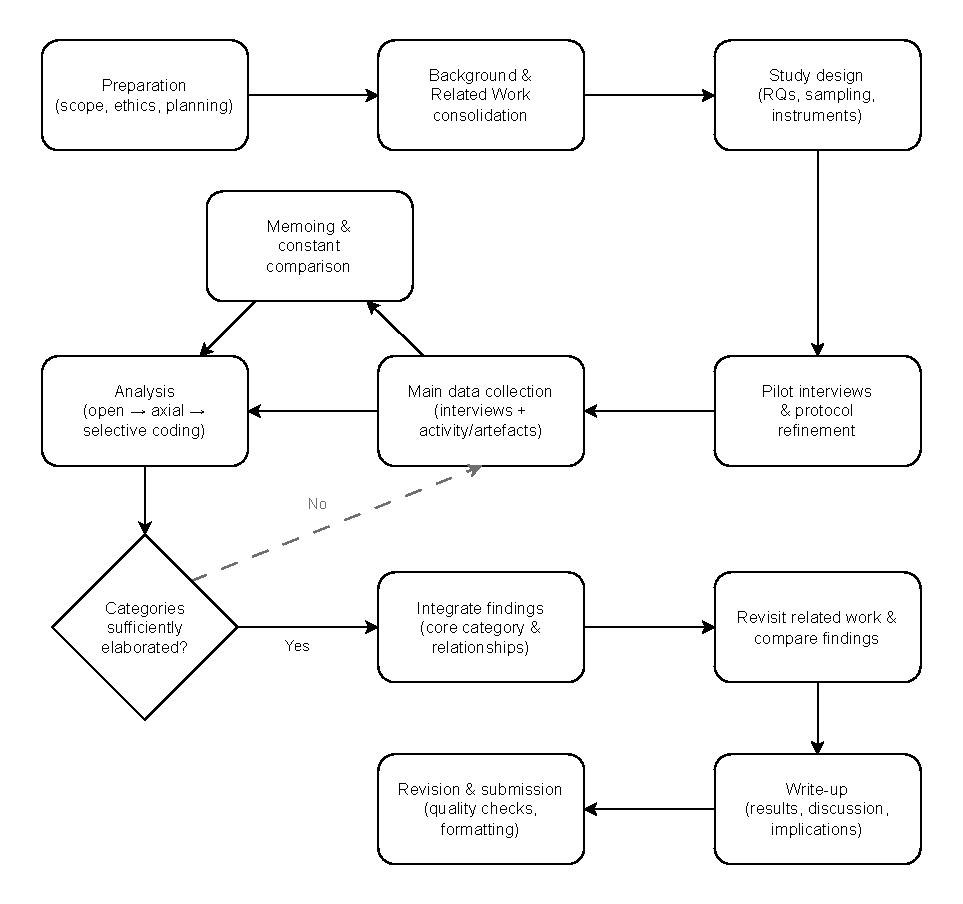
\includegraphics[width=\textwidth,height=0.85\textheight,keepaspectratio]{5-Figures/workflow_updated.pdf}
\caption{Planned thesis workflow (work plan).}
\label{fig:work_plan_flow}
\end{figure}


The workflow is intentionally iterative. After piloting, data collection and analysis proceed in parallel: interview prompts and sampling can be adjusted as categories emerge, and memoing supports continuous refinement of concepts. Iteration continues until categories are sufficiently elaborated to integrate an explanatory account, which is then consolidated into the final write-up and revisions.

\begin{figure}[H]
  \centering
  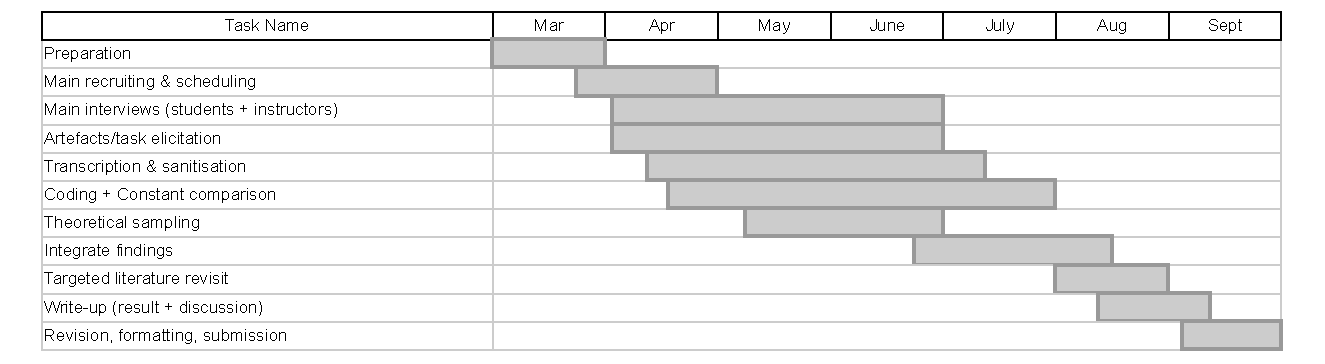
\includegraphics[width=\textwidth,height=0.85\textheight,keepaspectratio]{5-Figures/gantt.pdf}
\caption{Gantt chart of planned activities.}
\label{fig:gantt_chart}
\end{figure}

\noindent\textbf{Activity descriptions.}
\begin{itemize}
  \item \textbf{Preparation:} Finalise scope, instruments plan, consent and data handling procedures; obtain required approvals; refine interview guides for students and instructors; define prompts for task/artefact-anchored elicitation; adjust wording, ordering, timing, and probing strategy; refine the task/artefact elicitation flow.
  \item \textbf{Recruiting \& scheduling:} Recruit student and instructor participants; schedule sessions; manage consent and logistics.
  \item \textbf{Main interviews (students + instructors):} Conduct semi-structured interviews to elicit challenges, strategies/support needs, and socio-technical shaping factors.
  \item \textbf{Artefact/task elicitation:} Collect or walk through concrete models/tasks to ground accounts in situated examples (where feasible).
  \item \textbf{Transcription \& sanitisation:} Transcribe interviews; anonymise; prepare excerpts/artefact notes for analysis.
  \item \textbf{Coding \& constant comparison:} Perform iterative coding and memoing; compare across participants/courses/tools to refine categories.
  \item \textbf{Theoretical sampling (as needed):} Recruit additional participants or explore different contexts to elaborate emerging categories and test variation.
  \item \textbf{Integrate findings:} Consolidate categories around a core explanatory account and key relationships.
  \item \textbf{Targeted literature revisit:} Re-engage with the most relevant literature to position findings, highlight alignments/divergences, and sharpen implications.
  \item \textbf{Write-up:} Draft results, discussion, and implications/recommendations; connect findings to RQs.
  \item \textbf{Revision \& submission:} Quality checks, formatting, supervisor feedback incorporation, final edits, submission.
\end{itemize}
